\chapter{Background \& Literature Review} \label{ch:background-lit-review}
This chapter gives an introduction to the concepts of reaction diffusion and chemical computing,  as well as a review of the relevant literature.

\section{Reaction Diffusion}

Reaction diffusion is a field of science that has seen rapid innovations in the areas of image processing \citep{kuhnert1989image} and chemical computing \citep{dittrich2004chemical}. Among the numerous computing approaches, it has emerged as an alternative that takes advantage of the intrinsic ability of chemically reactive circuits to process information similar to that of computers. 

There are different reactions that produce oscillations, and the Belousov-Zhabotinsky (BZ) reaction is very popular. Others include the Briggs-Rauscher reaction \citep{de1982mechanistic}.
\section{Belousov-Zhabotinsky Reaction}
The Belousov-Zhabotinsky reaction \ref{fig:bz-reaction-pattern} was discovered by Boris Belousov in 1951 and later futher-studied and altered by Anatol Zhabotinsky in 1961. The reaction produces a chemical oscillation, which is a periodic change of the chemical concentration of two reactants. 
Belousov initially used malonic acid, potassium bromate, and cerium(IV) ions. Cerium was later changed to ferroin by Zhabotinsky in order to enhance the colour change of the reaction.
Ferroin was later changed for ruthenium(II) ions \citep{toth2006tris}, which is light sensitive, is the most common catalyst used today. The reaction is done in a petri dish that is about 2mm deep. 
It is an interesting reaction because it is one of the only reactions not requiring external energy to maintain. 
There are variations of it where all of the chemicals are not mixed together directly, but instead a catalyst is used to start the reaction.
This is very useful as it allows for starting and stopping the reaction at will, which enables the creation of a chemical computer.
A catalyst is a substance that increases the amount of excitement in a reaction, while not being consumed in the reaction itself.
One very common approach to control the reaction is to use light to control the excitability, a method commonly used by \cite{gorecki2003chemical}, where the catalyst in use is $\text{Ru(bpy)}_3\text{SO}_4$.

\begin{figure}[H]
    \centering
    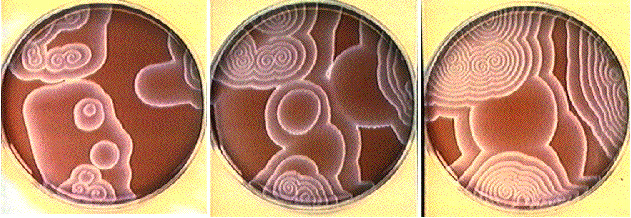
\includegraphics[width=0.75\linewidth]{images/BZWaves.jpg}
    \caption{Time-lapse of the Belousov-Zhabotinsky reaction in a petri dish done in the University of Stavanger}
    \label{fig:bz-reaction-pattern}
\end{figure}

\section{Chemical Computing}
Chemical computing makes use of chemical reactions to perform operations. 
\cite{Turing1952} is among the first to theoretically explore the field of Chemical Computing. 
His proposal was a model that could explain the creation of patterns in nature, such as the stripes on a zebra or the spots on a leopard.
Since then the field has seen a lot of exploration. One of the pioneers there is \cite{adamatzky2005reaction}, who has done a lot of work in the field. 
\cite{adamatzky2019brief} includes work on slime moulds that can solve mazes, both in real life and in simulations.

\section{Oregonator Model} 
The original Oregonator model uses 5 reactants: A, Y, X, B, and Z to form an oscillation. This project uses a more simplified and very popular model of the Oregonator, which makes use of only U and V as reactants and still accurately produces oscillations. 
\subsection{The Mathematics Behind the Oregonator Model}\label{sec:oregonator-math}
\cite{field2007oregonator} mathematical model illustrated by equation~\ref{eq:u-partial-t} and \ref{eq:v-partial-t}, which uses a set of differential equations developed to describe and mimic the behaviour of a real BZ reaction, by allowing for the calculation of the concentration of the reactants over time.
The Oregonator model is a used to simulate the Belousov-Zhabotinsky reaction, which is a chemical oscillator.

\begin{equation}
    \frac{\partial u}{\partial t} = \frac{1}{\epsilon} \left[ u - u^2 - (fv + \phi) \frac{u - q}{u + q} \right] + D_u \nabla^2 u
    \label{eq:u-partial-t}
\end{equation}
\begin{equation}
    \frac{\partial v}{\partial t} = u - v
    \label{eq:v-partial-t}
\end{equation}


These equations form the basis of the simulation, allowing for the exploration of dynamic chemical systems through computational methods.
The meaning of every part of the equation was discovered mostly through experimentation by me and not through research, but still serves as a great introduction to the model:
$u$ and $v$ are the concentrations of the reactants. The reason there is two of them is to create a two-step process in order to make an oscillation.
$\frac{u - q}{u + q}$, shown in Figure \ref{fig:u-q_u+q-graph}, where $q$ is set to a very small value is used to create a specific curve that controls how quickly the rate of the reaction $(fv + \phi)$ changes $u$, 
depending on its own concentration. As there is less activator chemical ($u$), the rate of the reaction is sped up because the term is negative, as it becomes exactly $q$, 
it starts to slow down the concentration until $u^2$ starts getting too big and starts slowing it down. 
As $u$ increases, $v$ increases as well, and if it reaches a cell where $u$ has a high concentration, 
it gets plugged into the equation and since the term $- (fv + \phi) \frac{u - q}{u + q}$ is negative, 
it rapidly shuts the value of $u$ all the way to 0 and $v$ follows, creating an oscillation.
Strictly speaking, the equation can work without $\frac{u - q}{u + q}$, but this term is crucial for the proper operation of the oscillation as it allows for the 
proper formation of the tail of the waves. The reason for that is exactly the non-linearity of the term, which allows the edges of the wave that have a lower concentration
to form outside of the bounds of the circuit because these parts of the circuit require extra help due to the negative impact of the illumination. Without that, the 
waves would still work just fine under no illumination, but as soon as they have to pass through a gate that is separated by light, they would die instantly and not be able to pass through.
$D_u \nabla^2$ is the concentration of the neighbouring cells that diffuse into the current cell, which adds dimentionality to the process because now the equation starts operating in 2D 
and every cell computes its own concentration based on the concentration of the cells around it. 
$\phi$ is external illumination that moulds the circuit where the reaction takes place by being set to either $\phi_{\text{active}}$ or $\phi_{\text{passive}}$, 
active meaning the reaction is allowed to happen, or passive where it's very difficult for $u$ to reach a critical concentration to start growing before it gets shut down by the second term of the reaction.
The reason that $u^2$ does not decrease the reaction in the beginning is that the values of the reactants is very small and being squared makes them even smaller, but as they grow, the decrease becomes more meaningful.
All of these parameters are set to specific values that are commonly used in literature in order to strike a difficult balance where the oscillation works in a way where chemical circuits are possible. 

\begin{figure}
    \centering
    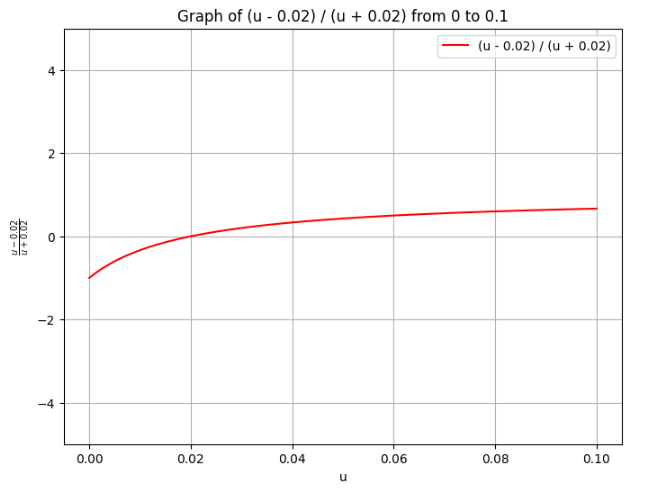
\includegraphics[width=0.75\linewidth]{images/Screenshot 2024-03-18 at 19.13.44.png}
    \caption{Graphical representation of the function $\frac{u - q}{u + q}$ showing how it influences the reaction rate in the Oregonator model}
    \label{fig:u-q_u+q-graph}
\end{figure}



There are two main uses of the Oregonator model when it comes to parameters that change the behaviour of the reaction, the first one creates waves that do not expand. 
They travel without changing their shape, and the second one creates waves that expand, which is the one used by this project.
Both ways have been shown to be able to create a Turing pattern, where the chemical circuits are vastly different, making use of the different properties of each model use-case.
\cite{stone2008coevolving} recreates an AND gate (Coincidence Detector) using the non-expanding wave method and the circuit is longer and more tunnel based. 
Most circuits in the expanding wave model are smaller as they rely on the intrinsic properties of the waves to hold more information in their shape, 
which is not possible in the non-expanding wave model where the waves are simpler are just travel along the non-illuminated gel material

\section{Motivation}
Although there is much potential there, most research focusses on building circuits in a simulation, such as \cite{StovoldJames2019RaGI}, versus in real life, such as \cite{gorecki2003chemical}. It is unclear whether exactly how the simulation maps to real life in terms of size and environmental factors that are likely to impact it. 
This is the reason for the focus of this project to be in between the real-life reactions and the simulations, looking at the impact of the imperfections of the environment on the computation.
